% \glsresetall
\chapter{Web Components} % Main chapter title
\label{Chapter4}

\lhead{Chapter 4. \emph{Web Components}}

\section{Web Components in general}

As in \ref{Chapter2} introduced, Web Components have the attribute of the Custom Element, via which the individuality of each registered tag is guaranteed.
Nonetheless to understand the actual functionality of Web Components, it is necessary to explain the other aspects of it.
The following section will introduce the other three standards of Web Components and their functions and showcase how exactly they serve a purpose for the context of the thesis.

\subsection{Shadow DOM}

The DOM (Document Object Model) represents the elements of a markup document in a tree-like structure, consisting of connected nodes. The commonly used markup language for websites is HTML. \cite{wc_shadow_dom}
The Shadow DOM is also a DOM, but is attached to the actual DOM of the document. Underneath it, elements can be defined the same way as they are in the regular DOM. The difference appears during the rendering of the document, when a page is loaded. The Shadow DOM elements are rendered separately from the DOM it is attached to.\cite{simon_thesis}

To understand the relationship between the two connected DOMs following terms have to be explained.

\begin{itemize}
	\item \textbf{Shadow host} - The attachment of the Shadow DOM to the normal DOM happens via a node inside the normal DOM.
	\item \textbf{Shadow tree} - Since the Shadow DOM is a DOM in itself, it consists of nodes in a tree-like structure.
	\item \textbf{Shadow boundary} - The Shadow DOM capsules its Shadow tree an renders it separately from the actual DOM. This encapsulated area defines where the Shadow DOM begins and ends.
	\item \textbf{Shadow root} - Just like a regular DOM a Shadow DOM has a root from where it originates.
\end{itemize} 

Figure \ref{fig:shadow_dom} visualizes the relations between the newly introduced terms.

\begin{figure}[!h]
	\centering
	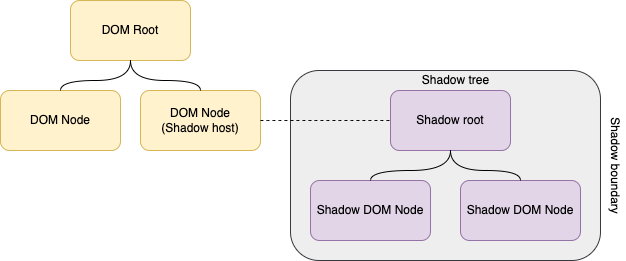
\includegraphics[width=1\textwidth]{Figures/shadow_dom.drawio.png}
	\caption{Shadow DOM architecture}
	\label{fig:shadow_dom}
\end{figure}

Through the isolation of the Shadow DOMs code, this standard offers a way to provide scoped HTML and CSS code to custom elements. As mentioned before, the nodes of the Shadow DOM are rendered separately. Therefore, styles, ids, names or even CSS classes and other configurations applied to a tag inside the Shadow DOM are not applied to the actual DOM.

Listing \ref{shadow_dom_definition} provides be a simple example.

\begin{lstlisting}[caption=Definition of a custom element using the Shadow DOM \cite{simon_thesis}, label=shadow_dom_definition]
<!DOCTYPE html> 
	...
	<body>
		<p>Plain</p> 
		<custom-element></custom-element>
		
		<script>
			class CustomElement extends HTMLElement {
				constructor() { 
					super();
					const shadow = this.attachShadow({mode: 'open'}); 
					shadow.innerHTML = `<style> p {color: red;} </style>`; 
					const shadowParagraph = document.createElement('p'); 
					shadowParagraph.textContent = 'Blue'; 
					shadow.appendChild(shadowParagraph);
				}
			}
			customElements.define('custom-element', CustomElement); 
			customElement = new CustomElement(); 
			console.log(customElement.shadowRoot)
		</script>
	</body>
</html>
\end{lstlisting}

The listing shows the usage of the Shadow DOM in combination with registering a custom element (named \texttt{custom-element}) using the customElements API which was explained in chapter \ref{Chapter2}.
The \texttt{script} tag of the snippet starts with creating a new HTML element called CustomElement. It is an extension to the HTMLElement class. This new element has the Shadow DOM attached to it. Therefore, it is the Shadow host in the DOM tree. Via the \texttt{innerHTML} attribute a Shadow DOM Node is created. In this case it is a styling for paragraphs,followed by the creation of a paragraph onto which the styling is applied. Additionally the text color of the paragraph is set to blue and lastly it is attached to the Shadow root.
The last three lines of the script, are the definition and registration of the new \texttt{custom-element}, the creation of a new \texttt{customElement} object and the output of the attached Shadow DOM in the console.

Now when looking at the body of the above snippet, it becomes visible that beside the \texttt{custom-element} another paragraph is defined in the document. Usually the styles defined in the \texttt{script} below would apply to this paragraph, too. Through the encapsulation of the two separate DOMs this is not the case. The paragraph defined in the body of the document will be completely unaffected by the changes applied to the paragraphs in the Shadow DOM.\cite{simon_thesis}

Now another configuration which is shown in the snippet is the \texttt{this.attachShadow({mode: 'open'})}. This mode property defines the visibility of the Shadow DOM to the browser. If set to \texttt{open}, the elements of the Shadow DOM can be inspected inside the sources. Thus, the \texttt{console.log(customElement.shadowRoot)} line would work if executed. 
If the mode would be set to \texttt{closed}  the \texttt{console.log()} command in line 20 would return \texttt{null}.\cite{simon_thesis}

This behavior is not meant to be used as a measure of security, since it can be overwritten. The Shadow DOM encapsulates every part of its DOM elements, that means HTML, CSS and JavaScript. The \texttt{document} object, available during runtime, stays the same for the regular DOM as for the Shadow DOM though. Therefore, each configuration done in the Shadow DOM via scripts can be easily overwritten from any other script in the document, thus the mode can be changed even if initially set to \texttt{closed}.\cite{shadow_dom_encapsulation} For Web Components in particular it is not recommended to use this mode at all, since it would make them less flexible for end users.\cite{wc_shadow_dom_google}

This feature can be used in combination with a component library like UI5 Web Components, to customize styles or appearances of individual components. Nonetheless, for the context of this thesis, it does not serve any purpose to actually avoid redundancies in a micro frontend landscape, instead it might even increase them. The encapsulation of code elements between the single components increases the isolation and thus it cannot be guaranteed that e.g. the same CSS class is not rendered in multiple different Shadow DOMs. Even though the redundancies would occur on code level and not on dependency level, they are redundancies nonetheless.

\subsection{HTML Template}

This standard offers a way to define reusable markup code. As a part of the HTML standard itself, the \texttt{template} tag is used to define templates. These are not rendered unless used by another element. Similar to \texttt{template}, \texttt{slot} serves the same purpose, but in a different way. Templates are defined HTML code snippets which can be cloned and inserted in other document elements or even elements rendered in the Shadow DOM.
Slots on the other hand serve as placeholder for either default markup texts or other DOM elements. Therefore, a template is a rather static piece of reusable HTML code, compared to slots.
Slot themselves are identified by their name, the content is inserted when the slot is addressed by its name.
Listings \ref{template_example} and \ref{slot_example} provide examples how exactly these two standards are used. \cite{wc_html_template_slots}

\begin{lstlisting}[caption=Definition and usage of the \texttt{template} standard \cite{wc_html_template_slots}, label=template_example]
<!-- Definition of the template -->
<template id="my-paragraph">
	<p>My paragraph</p>
</template>

<!-- Usage of the template in an Web Component -->
customElements.define('my-paragraph',
class extends HTMLElement {
	constructor() {
		super();
		let template = document.getElementById('my-paragraph');
		let templateContent = template.content;
		
		const shadowRoot = this.attachShadow({mode: 'open'})
		.appendChild(templateContent.cloneNode(true));
	}
});
\end{lstlisting}

It is important to note, that the defined template in the listing is not rendered unless somehow included in a DOM (either Shadow DOM or the regular DOM), via Java Script.

\begin{lstlisting}[language=HTML5, caption=Definition and usage of the \texttt{slot} standard \cite{wc_html_template_slots}, label=slot_example]
<!-- Definition of the slot -->
<p>
	<slot name="my-text">Default input</slot>
</p>

<!-- Usage of the slot in the markup document -->
<my-paragraph>
	<ul slot="my-text">
		<li>Some different input</li>
		<li>In a list!</li>
	</ul>
</my-paragraph>
\end{lstlisting}

As it can be seen in \ref{slot_example}, the \texttt{slot} definition has some default content defined. In the above case it´s a simple text. When the slot is used, this content is overwritten by the content in the element which is calling the \texttt{slot} by its name.
In that case the content is replaced by some list items.
Other than the templates, slots are always rendered if included in the markup via their respective names. The content which is rendered is depended on, if the default content is overwritten or not.

Even though slots are a HTML standard just as templates, their support for browsers is not always guaranteed. This is due to the fact, that compared to templates it is a rather new standard.

In combination these two standards offer a way to define flexible, reusable markup code for Web Components.\cite{wc_html_template_slots} 

When developing own Web Components for a micro frontend landscape, this aspect can be used to reduce repetitive HTML code elements by serving them a templates. But again this feature is not applicable when it comes to reducing redundant libraries in a micro frontend landscape. Redundant code snippets can be defined as reusable templates but not the actual libraries.

\subsection{ES Modules}

The last standard is not referred to by every source, but according to \cite{wc_specifications}, it is a stable part of the Web Components standard, via which Java Script modules can be defined and reused by other documents.
Thus the development of Web Components can be done in a modular way, making every component available to other documents, using the \texttt{type="module"} attribute.

\begin{lstlisting}[language=HTML5, caption=Importing modular Java Script documents into another \cite{wc_specifications}, label=es_modules_example]
<!-- Import of the JS Module -->
<script type="module" src="awesome-explosion.js"></script>
	...
<script type="module">
	import 'awesome-explosion.js';
	...
	import {awesomeExplosion} from '@awesome-things/awesome-explosion';
</script>

<!-- Usage of the newly imported module -->
<awesome-explosion>
	...
</awesome-explosion>
\end{lstlisting}

Listing \ref{es_modules_example} shows such an import. Assuming the \texttt{awesome-explosion.js} files contains the definition of an element called \texttt{awesome-explosion}, these lines enable the document to use this element.\cite{wc_specifications}

This feature is essential for the prototype developed, since via this aspect the components are made available to the landscape. The used Web Components are served as ES Modules to the landscape and are imported similarly as shown in \ref{es_modules_example}. Therefore, this aspect enables a component to be imported in multiple micro frontends as a module.

\section{Usage of Web Components in the Prototype}

The Web Components standard was partially used in the development of the prototype. This technology was used to embed the developed components as part of a compound view, using the corresponding feature in Luigi. \cite{luigi_wc} \cite{luigi_compound}
For development itself no UI application framework was used, which means all three compounds were developed using plain Java Script. The actual components used in the micro frontends of the compounds, were taken from a component library called UI5 Web Components. Each element in that library is in fact a Web Component.\cite{ui5_wc_github}
Consisting of the picked elements and under the usage of the scoping feature of the component library, the compounds where created. This made it possible to scope the tags of the UI5 Web Components.\cite{ui5_webcomponents_scoping}

\begin{lstlisting}[caption=Scoping feature used in the prototype, label=scoping_wc_prototype]
import { LuigiElement, html } 
from "@luigi-project/client/luigi-element.js";
import { setCustomElementsScopingSuffix } 
from "@ui5/webcomponents-base/dist/CustomElementsScope.js";
setCustomElementsScopingSuffix("placeholder");
import "@ui5/webcomponents/dist/Dialog.js";
import "@ui5/webcomponents/dist/Button.js";
[...]

export default class extends LuigiElement {
	constructor() {
		super();
		[...]
	render() {
		return html`
		<div>
			<div class="header">
				<h2>Products table - Version: placeholder</h2>
			</div>
			
			<ui5-table-placeholder id="ui5-table" 
			ui5-table sticky-column-header>
				<!-- Columns -->
				<ui5-table-column-placeholder 
					slot="columns" 
					style="width: 4rem">
					<span 
					style="line-height: 1.4rem">
						Product
					</span>
				</ui5-table-column-placeholder>
				
				[...]
				
			</ui5-table-placeholder>
		</div>`;
	}
}
\end{lstlisting}

Listing \ref{scoping_wc_prototype} shows the exact usage of the scoping feature. 
The imported \textit{setCustomElementsScopingSuffix} function enables to define a custom suffix to all UI5 Web Component elements, if not configured otherwise. Also, as it can be seen in the same listing, the suffix is set to \textit{placeholder} using the imported method 
\textit{setCustomElementsScopingSuffix("placeholder")}.
This is done for the sake of the experiment itself. It was intended to deploy six same or similar looking Web Components into the Luigi landscape to test how many redundancies occur. In addition it was meant to be tested how different versions of the same elements could be registered. For example the \textit{Bar} element in version \textit{1.0.1} is registered under same tag as the same element in version \textit{1.1.0}. This scenario has to be handled and the scoping feature is one way of doing so.
By defining a version suffix for the \textit{Bar} element tag, the browser can distinguish those elements.
In case of the prototype to create this exact scenario, one global tag suffix \textit{placeholder} was picked and later replaced. The replacement itself happened during the bundling of the project. The RollUp bundler provided the necessary functionality for that.
Inside the \texttt{rollup.config.js} several configurations were defined, which are shown in listing \ref{rollupconfigjs}.

\begin{lstlisting}[language=JavaScript, caption=Content of the \texttt{rollup.config.js}, label=rollupconfigjs]
imp\part{ort resolve from '@rollup/plugin-node-resolve';
import json from '@rollup/plugin-json';
import url from "@rollup/plugin-url";
import { terser } from "rollup-plugin-terser";
import replace from '@rollup/plugin-replace';
import { SameVersions } from './rollup_files/same_version';
import { DiffVersions } from './rollup_files/different_version';
import { MixedVersions } from './rollup_files/mixed_version';

let buildArray = [];

function aggregateConfigs() {
	for(let buildConfig of SameVersions) {
		buildArray.push(buildConfig);
	}
	
	for(let buildConfig of DiffVersions) {
		buildArray.push(buildConfig);
	}
	
	for(let buildConfig of MixedVersions) {
		buildArray.push(buildConfig);
	}
}

aggregateConfigs();

export default buildArray;
\end{lstlisting}

The configuration of the bundler was split into several Java Script files, to improve the readability of the configuration file itself. The content of such a file can be seen in \ref{rollupconfigfile}.

\begin{lstlisting}[language=JavaScript, caption=Actual configuration for the \texttt{rollup.config.js}, label=rollupconfigfile]
imp\part{ort resolve from '@rollup/plugin-node-resolve';
import resolve from '@rollup/plugin-node-resolve';
import json from '@rollup/plugin-json';
import url from "@rollup/plugin-url";
import { terser } from "rollup-plugin-terser";
import replace from '@rollup/plugin-replace';

export const MixedVersions = [
	// 1
	{
		input: 'src/tableView.js',
		output: {
			file: 'dist/tableViewMixedVersions1.js',
			format: 'es',
			compact: true
		},
		plugins: [
		replace({
			'placeholder': '0-9-0',
		}),
		terser(),
		resolve(),
		json(),
		url({
			limit: 0,
			include: [
			/.*assets\/.*\.json/,
			],
			emitFiles: true,
			fileName: "[name].[hash][extname]",
			publicPath: "\" + new URL(\".\", import.meta.url) + \"", // relative configuration for assets (TBD with UI5 Web Components team)
		})
		]
	},
	// 2
	{
		input: 'src/tableView.js',
		output: {
			file: 'dist/tableViewMixedVersions2.js',
			format: 'es',
			compact: true
		},
		plugins: [
		replace({
			'placeholder': '1-1-0',
		}),
		terser(),
		resolve(),
		json(),
		url({
			limit: 0,
			include: [
			/.*assets\/.*\.json/,
			],
			emitFiles: true,
			fileName: "[name].[hash][extname]",
			publicPath: "\" + new URL(\".\", import.meta.url) + \"", // relative configuration for assets (TBD with UI5 Web Components team)
		})
		]
	},
	[...]
]
\end{lstlisting}

The same file is used for bundling and each time it is bundled differently. The \texttt{replace} method of to configuration object replaces a string inside the input file. In this case the string \textit{placeholder} is first replaced with \textit{0-9-0} and in the second bundle configuration with \textit{1-1-0}. Also the files generated in the process are called differently, the first one is called \texttt{tableViewMixedVersions1.js} and the second \texttt{tableViewMixedVersions2.js}.
Even though the elements inside those files are actually the same, they are handled as differently, since their tags differ in the browser. Elements register for the first view are called for example \texttt{<ui5-bar-0-9-0>} and for the second then \texttt{<ui5-bar-1-1-0>}.

That means out of the same file, several differently bundled and named files were generated. Each one of the bundled files register the same elements under different tags which are therefore treated as new elements.

